% !TEX root = ../main.tex
\chapter{前置知识}
在学习微积分之前，我们需要先掌握几个工具。它们分别是行列式，向量，空间解析几何。有了这些，我们才能开启微积分的大门。我们只作最简单的介绍，掌握运算即可，不涉及过多的理论和证明。

\section{行列式}
\textbf{行列式}不仅是判断线性方程组有唯一解的关键量，也是后续计算向量叉乘的基础。本章将从二阶行列式出发，并将其推广到三阶。我们主要学习对角线法则和展开降阶两种计算方法，介绍行列式最基本的几条性质，如转置不变，交换变号等，并展示如何利用这些性质简化计算。本章内容限于二阶与三阶行列式，高阶行列式以及其他内容不作讨论。

\subsection{二阶行列式}

\begin{definition}{二阶行列式}{}
  由四个数排成两行两列，记作
  \[
  A = \begin{vmatrix}
    a & b \\
    c & d
  \end{vmatrix} = ad - bc
  \]
\end{definition}

我们可以这样理解：行列式 $A$ 的值等于主对角线（红色）的积减去副对角线（蓝色）的积。简记为“左上$\times$右下$-$右上$\times$左下”。

\[
A = \begin{vmatrix}
    \tikzmarknode{a}{a} & \tikzmarknode{b}{b} \\
    \tikzmarknode{c}{c} & \tikzmarknode{d}{d}
\end{vmatrix}
= \textcolor{red}{ad} - \textcolor{blue}{bc}
\begin{tikzpicture}[remember picture, overlay]
  \scoped[on background layer]{
    \draw[red, thick, opacity=0.5] (a.center) -- (d.center);
    \draw[blue, thick, opacity=0.5] (b.center) -- (c.center);
  }
\end{tikzpicture}
\]

\begin{myexample}
举例说明：设 $A = \begin{vmatrix}
    1 & 2 \\
    3 & 4
\end{vmatrix}$，求$A$。
$$
A = \begin{vmatrix}
    \tikzmarknode{a}{1} & \tikzmarknode{b}{2} \\
    \tikzmarknode{c}{3} & \tikzmarknode{d}{4}
\end{vmatrix}
= \textcolor{red}{1 \cdot 4} - \textcolor{blue}{2 \cdot 3} =\textcolor{red}{4}-\textcolor{blue}{6}=-2
\begin{tikzpicture}[remember picture, overlay]
  \scoped[on background layer]{
    \draw[red, thick, opacity=0.5] (a.center) -- (d.center);
    \draw[blue, thick, opacity=0.5] (b.center) -- (c.center);
  }
\end{tikzpicture}
$$
\end{myexample}

这就是二阶行列式的定义及其计算方法。

\subsection{三阶行列式}
与二阶行列式类似，我们给出三阶行列式的定义：
\begin{definition}{三阶行列式}{}
  由九个数排成三行三列，记作
  $$
  A = \begin{vmatrix}
    a & b & c \\
    d & e & f \\
    g & h & i
  \end{vmatrix} = aei + bfg + cdh - ceg - bdi - afh
  $$
\end{definition}
我们可以这样理解：行列式 $A$ 的值等于三条主对角线（红色）的积之和减去三条副对角线（蓝色）的积之和。

\[
A = \begin{vmatrix}
    \tikzmarknode{a}{a} & \tikzmarknode{b}{b} & \tikzmarknode{c}{c} \\
    \tikzmarknode{d}{d} & \tikzmarknode{e}{e} & \tikzmarknode{f}{f} \\
    \tikzmarknode{g}{g} & \tikzmarknode{h}{h} & \tikzmarknode{i}{i}
\end{vmatrix}
= \textcolor{red}{aei} + \textcolor{red}{bfg} + \textcolor{red}{cdh} - \textcolor{blue}{ceg} - \textcolor{blue}{afh} - \textcolor{blue}{bdi}
\begin{tikzpicture}[remember picture, overlay]
  \scoped[on background layer]{
    % 三条主对角线（红色，半透明）
    \draw[red, thick, opacity=0.5]
      (a.center) -- (e.center) -- (i.center);
    \draw[red, thick, opacity=0.5]
      (b.center) -- (f.center) -- (g.center);
    \draw[red, thick, opacity=0.5]
      (c.center) -- (d.center) -- (h.center);
    % 三条副对角线（蓝色，半透明）
    \draw[blue, thick, opacity=0.5]
      (c.center) -- (e.center) -- (g.center);
    \draw[blue, thick, opacity=0.5]
      (a.center) -- (f.center) -- (h.center);
    \draw[blue, thick, opacity=0.5]
      (b.center) -- (d.center) -- (i.center);
  }
\end{tikzpicture}
\]

显然，这种方法是非常难记住的，因此我们有一个相对简单的方法来计算三阶行列式，叫做展开降阶法：
$$A = a \begin{vmatrix}
    e & f \\
    h & i
  \end{vmatrix} - b \begin{vmatrix}
    d & f \\
    g & i
  \end{vmatrix} + c \begin{vmatrix}
    d & e \\
    g & h
  \end{vmatrix}$$

其中，$a$ 后面的二阶行列式叫做 $a$ 的余子式，$b$ 后面的二阶行列式叫做 $b$ 的余子式，$c$ 后面的二阶行列式叫做 $c$ 的余子式。我们可以选择任意一行或者一列来展开，结果都是一样的。

怎么理解呢？我们还是先看一下这个三阶行列式：
\[
A = \begin{vmatrix}
    a & b & c \\
    d & e & f \\
    g & h & i
  \end{vmatrix}
\]

先固定$a$所在的行和列不动，暂时忽略。剩下的数看作一个二阶行列式（ $a$ 的余子式），计算这个二阶行列式，结果再与$a$相乘。

\[
A = \begin{vmatrix}
    a & \blacksquare & \blacksquare \\
    \blacksquare & e & f \\
    \blacksquare & h & i
  \end{vmatrix}
  = a \begin{vmatrix}
    e & f \\
    h & i
  \end{vmatrix}
  \cdots
\]

同理，再固定$b$所在的行和列不动，暂时忽略。剩下的数看作一个二阶行列式（ $b$ 的余子式），计算这个二阶行列式，结果再与$b$相乘。\textbf{注意：}这一项的符号是负的。

\[
A = \begin{vmatrix}
    \blacksquare & b & \blacksquare \\
    d & \blacksquare & f \\
    g & \blacksquare & i
  \end{vmatrix}
  = a \begin{vmatrix}
    e & f \\
    h & i
  \end{vmatrix}
  - b \begin{vmatrix}
    d & f \\
    g & i
    \end{vmatrix}
    \cdots
\]

最后，固定$c$所在的行和列不动，暂时忽略。剩下的数看作一个二阶行列式（ $c$ 的余子式），计算这个二阶行列式，结果再与$c$相乘。\textbf{注意：}这一项的符号是正的。

\[
A = \begin{vmatrix}
    \blacksquare & \blacksquare & c \\
    d & e & \blacksquare \\
    g & h & \blacksquare
  \end{vmatrix}
  = a \begin{vmatrix}
    e & f \\
    h & i
  \end{vmatrix}
  - b \begin{vmatrix}
    d & f \\
    g & i
    \end{vmatrix}
  + c \begin{vmatrix}
    d & e \\
    g & h
  \end{vmatrix}
\]

由此，我们得到了三阶行列式的展开降阶法：
\begin{theorem}{三阶行列式的展开降阶法}{}
  $$A =  \begin{vmatrix}
    a & b & c \\
    d & e & f \\
    g & h & i
  \end{vmatrix} =
  a \begin{vmatrix}
    e & f \\
    h & i
  \end{vmatrix} - b \begin{vmatrix}
    d & f \\
    g & i
  \end{vmatrix} + c \begin{vmatrix}
    d & e \\
    g & h
  \end{vmatrix}$$
\end{theorem}

\begin{myexample}
  举例说明：设 $A = \begin{vmatrix}
    1 & 2 & 3 \\
    4 & 5 & 6 \\
    7 & 8 & 9
  \end{vmatrix}$，求$A$。

  \begin{align*}
    A &= 1 \cdot \begin{vmatrix} 5 & 6 \\ 8 & 9 \end{vmatrix}
        - 2 \cdot \begin{vmatrix} 4 & 6 \\ 7 & 9 \end{vmatrix}
        + 3 \cdot \begin{vmatrix} 4 & 5 \\ 7 & 8 \end{vmatrix} \\
      &= 1 \cdot (5\cdot 9 - 6\cdot 8) - 2 \cdot (4\cdot 9 - 6\cdot 7) + 3 \cdot (4\cdot 8 - 5\cdot 7) \\
      &= 1 \cdot (45 - 48) - 2 \cdot (36 - 42) + 3 \cdot (32 - 35) \\
      &= 1 \cdot (-3) - 2 \cdot (-6) + 3 \cdot (-3) \\
      &= -3 + 12 - 9 \\
      &= 0
  \end{align*}
\end{myexample}

实际上，由降阶法，我们可以计算更高阶的行列式，但本章不作讨论。

\subsection{行列式的简单性质}
行列式有很多性质，这里我们只列举几个最基本的性质，计算的时候可能会用到它们。

\begin{theorem}{行列转置}{}
\[
\begin{vmatrix}
a_1 & a_2 & a_3 \\
b_1 & b_2 & b_3 \\
c_1 & c_2 & c_3
\end{vmatrix}
=
\begin{vmatrix}
a_1 & b_1 & c_1 \\
a_2 & b_2 & c_2 \\
a_3 & b_3 & c_3
\end{vmatrix}
\]
\textbf{推论}：若对行有成立的性质，对列也必成立。因为转置后行列式的值不变，这意味着\textbf{行与列的地位完全对称}。
\end{theorem}

\begin{theorem}{交换变号}{}
\[
\begin{vmatrix}
a_1 & a_2 & a_3 \\
b_1 & b_2 & b_3 \\
c_1 & c_2 & c_3
\end{vmatrix}
= -
\begin{vmatrix}
b_1 & b_2 & b_3 \\
a_1 & a_2 & a_3 \\
c_1 & c_2 & c_3
\end{vmatrix}
\]
\textbf{推论：}若有两行（列）相同，行列式为$0$。因为交换相同的两行，行列式既要等于自己，又要变号，只能是$0$。
\end{theorem}

\begin{theorem}{提取公因子}{}
\[
\begin{vmatrix}
ka_1 & ka_2 & ka_3 \\
b_1 & b_2 & b_3 \\
c_1 & c_2 & c_3
\end{vmatrix}
= k
\begin{vmatrix}
a_1 & a_2 & a_3 \\
b_1 & b_2 & b_3 \\
c_1 & c_2 & c_3
\end{vmatrix}
\]
\textbf{推论：}若某一行（列）全为$0$，行列式为$0$（相当于提出因子$0$）。若两行（列）成比例，提出比例因子后剩下两行相同，行列式也为$0$。
\end{theorem}

这里我们不给出例子。具体计算的时候自然会用到。

\section{空间向量}
这个章节中，我们假定读者有基础的高中知识，已经学习过平面向量的数乘，点积，坐标表示等内容，因此我们直接从向量的叉积开始。

\subsection{向量的叉积}
\begin{definition}{向量的叉积}{}
设 $\vec{a} = (a_1, a_2, a_3)$ 和 $\vec{b} = (b_1, b_2, b_3)$ 是三维空间中的两个向量，夹角为 $\theta (0 \leq \theta \leq \pi)$，记它们的叉积（又称向量积）为$\vec{c}$，则$\vec{c}$定义为：
\[\vec{c}=
\vec{a} \times \vec{b}
= \begin{vmatrix}
\vec{i} & \vec{j} & \vec{k} \\
a_1 & a_2 & a_3 \\
b_1 & b_2 & b_3
\end{vmatrix}
= (a_2 b_3 - a_3 b_2,\; a_3 b_1 - a_1 b_3,\; a_1 b_2 - a_2 b_1)
\]
其中 $\vec{i}, \vec{j}, \vec{k}$ 分别是沿 $x,y,z$ 轴正方向的单位向量。

$\vec{c}$的模长为$|\vec{c}|=|\vec{a}||\vec{b}|\sin\theta$，方向垂直于 $\vec{a}$ 和 $\vec{b}$ 所在的平面。具体指向由右手定则确定。
\end{definition}

\begin{definition}{右手定则}{}
  伸出右手，四指指向第一个向量 $\vec{a}$ 的方向，然后向第二个向量 $\vec{b}$沿较小的夹角（$\leq \pi$） 弯曲握拢，此时大拇指所指的方向就是 $\vec{a} \times \vec{b}$ 的方向。
\end{definition}

应当注意，向量的叉积是一个向量，而不是一个数。叉积的模长等于由这两个向量构成的平行四边形的面积。特殊地，若$\vec{a} \times \vec{b} = \vec{0}$，则表示两向量共线。

\begin{myexample}
  举例说明：设 $\vec{a} = (0, 1, 0)$ 和 $\vec{b} = (0, 0, 1)$，记 $\vec{c} = \vec{a} \times \vec{b}$，求 $\vec{c}$ 的方向。

  我们画一个草图展示 $\vec{a}$（红色）、$\vec{b}$（蓝色）以及它们的叉积 $\vec{c}$（绿色）的关系。

    \begin{center}
    \begin{tikzpicture}[
      scale=1.2,
      x={(-0.5cm,-0.5cm)},
      y={(1cm,0cm)},
      z={(0cm,1cm)},
      >=stealth
    ]
      % 坐标轴
      \draw[->] (-0.5,0,0) -- (2.5,0,0) node[below right] {$x$};
      \draw[->] (0,-0.5,0) -- (0,2.5,0) node[above left] {$y$};
      \draw[->] (0,0,0.5) -- (0,0,2.5) node[above] {$z$};

      \draw[red, very thick, ->] (0,0,0) -- (0,1.8,0) node[below right] {$\vec{a}=(0,1,0)$};

      \draw[blue, very thick, ->] (0,0,0) -- (0,0,1.8) node[above right] {$\vec{b}=(0,0,1)$};

      \draw[green!60!black, very thick, ->] (0,0,0) -- (1.8,0,0) node[below right] {$\vec{c}=(1,0,0)$};

      % 右手定则弧线
      \begin{scope}[canvas is yz plane at x=0]
        \draw[->, gray, thick]
          (0.6,0) arc[start angle=0, end angle=90, radius=0.6cm]
          node[midway, above right] {右手四指};
      \end{scope}
    \end{tikzpicture}
  \end{center}

  从图中可看出，$\vec{a}$ 沿 $y$ 轴，$\vec{b}$ 沿 $z$ 轴，右手四指从 $y$ 转向 $z$ 时，大拇指指向 $x$ 轴正方向，即 $\vec{c}$ 的方向。
\end{myexample}

我们很快发现，如果令$\vec{c} = \vec{b} \times \vec{a}$，此时$\vec{c}$ 的方向与 $\vec{a} \times \vec{b}$ 的方向相反。这是因为交换了 $\vec{a}$ 和 $\vec{b}$ 的位置，右手四指从 $z$ 转向 $y$ 时，大拇指指向 $x$ 轴负方向。由此我们可以得出叉积的一条重要性质：
\begin{theorem}{叉积的反对称性}{}
\[
\vec{a} \times \vec{b} = -(\vec{b} \times \vec{a})
\]
\end{theorem}

\begin{myexample}
  举例说明：设 $\vec{a} = (1, 2, 3)$ 和 $\vec{b} = (4, 5, 6)$，求 $\vec{a} \times \vec{b}$和$\vec{b} \times \vec{a}$。

  \begin{align*}
    \vec{a} \times \vec{b}
    &= \begin{vmatrix}
       \vec{i} & \vec{j} & \vec{k} \\
       1 & 2 & 3 \\
       4 & 5 & 6
       \end{vmatrix} \\
    &= \vec{i} \begin{vmatrix} 2 & 3 \\ 5 & 6 \end{vmatrix}
       - \vec{j} \begin{vmatrix} 1 & 3 \\ 4 & 6 \end{vmatrix}
       + \vec{k} \begin{vmatrix} 1 & 2 \\ 4 & 5 \end{vmatrix} \\
    &= \vec{i}(2\cdot6 - 3\cdot5) - \vec{j}(1\cdot6 - 3\cdot4) + \vec{k}(1\cdot5 - 2\cdot4) \\
    &= \vec{i}(12 - 15) - \vec{j}(6 - 12) + \vec{k}(5 - 8) \\
    &= -3\vec{i} + 6\vec{j} - 3\vec{k} \\
    &= (-3,\; 6,\; -3)
    \end{align*}

    \begin{align*}
    \vec{b} \times \vec{a}
    &= \begin{vmatrix}
       \vec{i} & \vec{j} & \vec{k} \\
       4 & 5 & 6 \\
       1 & 2 & 3
       \end{vmatrix} \\
    &= \vec{i} \begin{vmatrix} 5 & 6 \\ 2 & 3 \end{vmatrix}
       - \vec{j} \begin{vmatrix} 4 & 6 \\ 1 & 3 \end{vmatrix}
       + \vec{k} \begin{vmatrix} 4 & 5 \\ 1 & 2 \end{vmatrix} \\
    &= \vec{i}(5\cdot3 - 6\cdot2) - \vec{j}(4\cdot3 - 6\cdot1) + \vec{k}(4\cdot2 - 5\cdot1) \\
    &= \vec{i}(15 - 12) - \vec{j}(12 - 6) + \vec{k}(8 - 5) \\
    &= 3\vec{i} - 6\vec{j} + 3\vec{k} \\
    &= (3,\; -6,\; 3)
    \end{align*}
\end{myexample}

计算过程中，根据行列式的交换变号性，我们也能看出叉积的反对称性。

\subsection{向量的混合积}
向量的混合积并不常用，我们简单带过。

\begin{definition}{向量的混合积}{}
设 $\vec{a} = (a_1, a_2, a_3)$，$\vec{b} = (b_1, b_2, b_3)$ 和 $\vec{c} = (c_1, c_2, c_3)$ 是三维空间中的三个向量，记它们的混合积为 $[\vec{a}, \vec{b}, \vec{c}]$，则 $[\vec{a}, \vec{b}, \vec{c}]$ 定义为：
\[ [\vec{a}, \vec{b}, \vec{c}] = \vec{a} \cdot (\vec{b} \times \vec{c}) = \begin{vmatrix}
a_1 & a_2 & a_3 \\
b_1 & b_2 & b_3 \\
c_1 & c_2 & c_3
\end{vmatrix} \]
\end{definition}

应当注意，向量的混合积是一个数，而不是一个向量。混合积的绝对值等于由这三个向量构成的平行六面体的体积。特殊地，若 $[\vec{a}, \vec{b}, \vec{c}] = 0$，则表示这三个向量共面。

\section{空间解析几何}
这一节开始难度会升高。我们将介绍空间中的曲线和曲面。我们依旧假定读者有基础的高中知识，已经学习过平面解析几何和空间立体几何的基本内容，因此我们直接从空间解析几何的内容开始。

\subsection{平面方程}

在空间中，确定一个平面最自然的方式是：给定平面上的一个点，以及垂直于平面的方向，这个方向由一个法向量给出。这种确定平面的方法只需要一个点和一个法向量。因此，我们可以给出这样的定义：

\begin{definition}{平面的点法式方程}{}
设 $\Sigma$ 是空间中的一个平面，$P_0(x_0,y_0,z_0)$ 是 $\Sigma$ 上的一个点，$\vec{n} = (A,B,C)$ 是 $\Sigma$ 的一个法向量，则 $\Sigma$ 的平面方程为：
$$A(x-x_0)+B(y-y_0)+C(z-z_0)=0$$
\end{definition}

如果将点法式方程展开，写成$Ax + By + Cz + D = 0$的形式，我们便得到了一般式方程：

\begin{definition}{平面的一般式方程}{}
设 $\Sigma$ 是空间中的一个平面，则 $\Sigma$ 的一般式方程为：
$$Ax + By + Cz + D = 0$$
\end{definition}

由一般式可以看出，$\vec{n} = (A,B,C)$仍然是平面的一个法向量。因此，确定了法向量，就确定了平面的朝向。

\begin{myexample}
举例说明：求过点$P_0=(1,2,3)$且法向量为$\vec{n}=(4,5,6)$的平面方程。

$P_0=(1,2,3)$，$\vec{n}=(4,5,6)$，我们得到：
\[
4(x-1)+5(y-2)+6(z-3)=0
\]

因此，平面 $\Sigma$ 的方程为：
\[
4x+5y+6z-32=0
\]
\end{myexample}

\begin{myexample}
举例说明：已知$A(1,1,1),B(1,2,3),C(3,3,3)$，求过线段$AB,BC$的平面方程。

先计算向量$\overrightarrow{AB},\overrightarrow{BC}$：
\[
\overrightarrow{AB} = (1-1,\,2-1,\,3-1) = (0,\,1,\,2)
\]
\[
\overrightarrow{BC} = (3-1,\,3-2,\,3-3) = (2,\,1,\,0)
\]

两向量不平行，因此 $A,B,C$ 三点不共线，可唯一确定一个平面。

平面的法向量 $\vec{n}$ 可用向量叉积求得：
\[
\vec{n} = \overrightarrow{AB} \times \overrightarrow{BC}
= \begin{vmatrix}
\vec{i} & \vec{j} & \vec{k} \\
0 & 1 & 2 \\
2 & 1 & 0
\end{vmatrix}
= \vec{i}(1\cdot0 - 2\cdot1) - \vec{j}(0\cdot0 - 2\cdot2) + \vec{k}(0\cdot1 - 1\cdot2)
= (-2,\,4,\,-2)
\]

取简化形式 $\vec{n} = (1,\,-2,\,1)$。

由点法式，代入点 $A(1,1,1)$ 得：
\[
1\cdot(x-1) + (-2)\cdot(y-1) + 1\cdot(z-1) = 0
\]

展开并整理：
\[
x - 2y + z = 0
\]

\begin{center}
  \begin{tikzpicture}[scale=1.4, line join=round]
  \tdplotsetmaincoords{60}{110}
  \begin{scope}[tdplot_main_coords]

    % 坐标轴（略大于三角形范围）
    \draw[->] (0,0,0) -- (3,0,0) node[above] {$x$};
    \draw[->] (0,0,0) -- (0,3,0) node[above] {$y$};
    \draw[->] (0,0,0) -- (0,0,3) node[left] {$z$};

    % 三角形 ABC 填充
    \fill[blue!15, opacity=0.7] (1,1,1) -- (1,2,3) -- (3,3,3) -- cycle;
    \draw[thick] (1,1,1) -- (1,2,3) -- (3,3,3) -- cycle;

    % 三个顶点
    \filldraw (1,1,1) circle (2pt) node[below left]  {$A(1,1,1)$};
    \filldraw (1,2,3) circle (2pt) node[above left]  {$B(1,2,3)$};
    \filldraw (3,3,3) circle (2pt) node[right]        {$C(3,3,3)$};

    % 平面方程
    \node at (3,4,4) [below] {$x-2y+z=0$};

  \end{scope}
\end{tikzpicture}
\end{center}

\end{myexample}

\subsection{空间直线方程}
空间中的直线可以看作两个不平行的平面的交线，因此我们可以用两个平面方程联立来表示一条直线。但更方便的方式是使用点向式方程。

\begin{definition}{直线的方向向量}{}
在空间（或平面）中，如果一条直线$L$已经确定，那么任何一个与$L$平行的非零向量，都称为这条直线的一个方向向量。
\end{definition}

显然，一条直线有无数个方向向量。我们可以通过一点和一个方向向量确定一条空间直线。


\begin{definition}{直线的点向式方程}{}
设直线 $L$ 经过点 $P_0(x_0,y_0,z_0)$，且方向向量为 $\vec{s}=(m,n,p)$（其中 $m,n,p$ 不全为零），则 $L$ 的方程为：
\[
\frac{x-x_0}{m} = \frac{y-y_0}{n} = \frac{z-z_0}{p}
\]
特别的，如果某个分母为零，则相应的分子也为零，表示该坐标恒定。例如$m=0$时，直线方程变为：

$$L: \begin{cases}\frac{y-y_0}{n} = \frac{z-z_0}{p}\\x=x_0\end{cases}$$

此时直线垂直于$x$轴。

\end{definition}

因此，已知直线上一点以及直线的一个方向向量，就可以求出空间直线的方程。已知直线的点向式方程，我们可以读出直线上一点与直线的一个方向向量。

\begin{myexample}
  举例说明：已知直线$L$过$P_0(1,2,3)$，其中一个方向向量为$\vec{s}=(4,5,6)$，求$L$的方程。

  由点向式方程可得：
  \[
  \frac{x-1}{4} = \frac{y-2}{5} = \frac{z-3}{6}
  \]
\end{myexample}

由点向式方程我们可以看出，$\frac{x-x_0}{m} , \frac{y-y_0}{n} , \frac{z-z_0}{p}$这三个分数都相等，那么我们可以引入一个参数$t$（$t\in\mathbb{R}$），令$\frac{x-x_0}{m} = \frac{y-y_0}{n} = \frac{z-z_0}{p} = t$，将$m,n,p$都乘到等式右边，则有：

$$\begin{cases}
  x-x_0=mt\\
  y-y_0=nt\\
  z-z_0=pt
\end{cases}$$

这就得到了直线的参数式方程：

\begin{definition}{直线的参数式方程}{}
设直线 $L$ 经过点 $P_0(x_0,y_0,z_0)$，且方向向量为 $\vec{s}=(m,n,p)$（其中 $m,n,p$ 不全为零），则 $L$ 的方程为：
$$L: \begin{cases}
  x=mt+x_0\\
  y=nt+y_0\\
  z=pt+z_0
\end{cases}$$

其中$t\in\mathbb{R}$。

特别的，如果方向向量某个分量为零，则该坐标恒定。例如$m=0$时，直线方程变为：

$$L: \begin{cases}
  x=x_0\\
  y=nt+y_0\\
  z=pt+z_0
\end{cases}$$

此时直线垂直于$x$轴。
\end{definition}

\begin{myexample}
  举例说明：已知空间直线 \(L\) 经过两点 \(A(2, -1, 5)\) 和 \(B(8, -1, 1)\)，求直线 \(L\) 的点向式方程和参数式方程。

  先求\(\overrightarrow{AB}\)：\(\overrightarrow{AB} = (6,\ 0,\ -4)\)。取简化形式 \(\overrightarrow{AB} = (3,0,-2)\)。

  则已知 \(A(2, -1, 5)\)为直线上一点，\(\vec{s} = (3,0,-2)\) 为直线的一个方向向量。

  由点向式方程可得：

  \[
  L: \begin{cases}
  \frac{x-2}{3} = \frac{z-5}{-2}\\
  y = -1\end{cases}
  \]

  由参数式方程可得：

  \[
  L: \begin{cases}
    x = 2 + 3t \\
    y = -1 \\
    z = 5 - 2t
  \end{cases}
  \]

\end{myexample}

这个例子也说明了两点确定一条直线。

\subsection{曲面方程}
类比平面中的曲线方程，我们可以推断曲面方程也由类似的结构组成。本节中仅讨论二次曲面，即方程中坐标的最高次数是$2$的曲面。因此，本节需要一定的解析几何中二次曲线的基础。

面对一个复杂的二次曲面方程，直接想象它的空间形状并不容易。我们通常采用截痕法讨论：

\begin{definition}{截痕法}{}
用一族\textbf{相互平行}的平面与曲面相交，得到一系列平面截线。通过分析这些截线连续变化时的形状、大小、位置和变化趋势，从而分析出该曲面的整体空间形态与结构特征。
\end{definition}

怎么理解呢？假设你现在是脑科医生，为病人做了一个CT检查。你将CT检查得到的图片堆叠起来，终于把病人的脑子看清楚了——CT检查和截痕法的底层逻辑是一样的，二次曲面就像病人的脑子。CT检查是一层层扫描得到图片，然后再拼起来，截痕法是用平行平面一层层与曲面相交，得到一条条交线，然后再将这些交线拼起来，就能大致分析出曲面的形状。

\begin{myexample}
  举例说明：描述曲面$\Sigma: x^2+y^2+z^2=9$的形状。

  我们先用平面$z=0$截这个曲面，那么交线就必须同时满足$z=0$和$x^2+y^2+z^2=9$这两个方程。我们把$z=0$带进$\Sigma$的方程里，得到$x^2+y^2=9$，也就是说：

  在$z=0$时，$\Sigma$是以原点为圆心，半径为$3$的圆。

  我们再用平行的平面$z=1$截这个曲面，那么交线就必须同时满足$z=1$和$x^2+y^2+z^2=9$这两个方程。我们再把$z=1$带进$\Sigma$的方程里，得到$x^2+y^2=8$，也就是说：

  在$z=1$时，$\Sigma$是以$(0,0,1)$为圆心，半径为$2\sqrt{2}$的圆。

  同理：在$z=2$时，$\Sigma$是以$(0,0,2)$为圆心，半径为$\sqrt{5}$的圆。

  在$z=3$时，$\Sigma$是一个点，点的坐标为$(0,0,3)$。

  在$z=4$时，$\Sigma$不存在。

  同理，在$z$轴下方，我们能得到：

  在$z=-1$时，$\Sigma$是以$(0,0,-1)$为圆心，半径为$2\sqrt{2}$的圆。

  在$z=-2$时，$\Sigma$是以$(0,0,-2)$为圆心，半径为$\sqrt{5}$的圆。

  在$z=-3$时，$\Sigma$是一个点，点的坐标为$(0,0,-3)$。

  在$z=-4$时，$\Sigma$不存在。

\begin{center}
  \begin{tikzpicture}[scale=1.2]
  \tdplotsetmaincoords{54.7356}{135}
  \begin{scope}[tdplot_main_coords]
    \def\R{3}
    \def\rI{2.828}   % sqrt(8)
    \def\rII{2.236}  % sqrt(5)

    % ---- 虚线区间参数----
    \def\zMinusTwoDashStart{125.90}    % z=-2
    \def\zMinusTwoDashEnd{324.01}
    \def\zMinusOneDashStart{142.18}  % z=-1
    \def\zMinusOneDashEnd{307.82}
    \def\zZeroDashStart{155.70}        % z=0
    \def\zZeroDashEnd{294.30}
    \def\zOneDashStart{173.68}
    \def\zOneDashEnd{276.32}

    % 坐标轴
    \draw[->, black] (0,0,0) -- (4,0,0) node[below left] {$x$};
    \draw[->, black] (0,0,0) -- (0,4,0) node[below right] {$y$};
    \draw[->, black] (0,0,3) -- (0,0,4) node[above] {$z$};
    \draw[black, dashed] (0,0,0) -- (0,0,-3);
    \draw[black, dashed] (0,0,0) -- (0,0,3);

    % 球轮廓
    \draw[black] (0,0,3) -- (0,0,4);
    \draw[black] (0,0,-3) -- (0,0,-4);

    % ---------- 各截面圆 ----------

    % z=-3 顶点
    \filldraw[black] (0,0,-3) circle (1pt) node[below] {$(0,0,-3)$};

    % z = -2
    \fill[green!20, opacity=0.5] plot[variable=\t, domain=0:360, samples=72]
      ({\rII*cos(\t)},{\rII*sin(\t)},-2);
    \draw[green!50!black, thick, dashed] plot[variable=\t, domain=\zMinusTwoDashStart:\zMinusTwoDashEnd, samples=80]
      ({\rII*cos(\t)},{\rII*sin(\t)},-2);
    \draw[green!50!black, thick] plot[variable=\t, domain=\zMinusTwoDashEnd:360, samples=40]
      ({\rII*cos(\t)},{\rII*sin(\t)},-2);
    \draw[green!50!black, thick] plot[variable=\t, domain=0:\zMinusTwoDashStart, samples=30]
      ({\rII*cos(\t)},{\rII*sin(\t)},-2);
    \node[green!50!black] at ({\rII*cos(90)}, {\rII*sin(90)},-2) [below right] {$z=-2$};
    \filldraw[black] (0,0,-2) circle (1pt) node[below] {$(0,0,-2)$};

    % z = -1
    \fill[blue!20, opacity=0.5] plot[variable=\t, domain=0:360, samples=72]
      ({\rI*cos(\t)},{\rI*sin(\t)},-1);
    \draw[blue, thick, dashed] plot[variable=\t, domain=\zMinusOneDashStart:\zMinusOneDashEnd, samples=90]
      ({\rI*cos(\t)},{\rI*sin(\t)},-1);
    \draw[blue, thick] plot[variable=\t, domain=\zMinusOneDashEnd:360, samples=40]
      ({\rI*cos(\t)},{\rI*sin(\t)},-1);
    \draw[blue, thick] plot[variable=\t, domain=0:\zMinusOneDashStart, samples=30]
      ({\rI*cos(\t)},{\rI*sin(\t)},-1);
    \node[blue] at ({\rI*cos(60)}, {\rI*sin(60)},-1) [above] {$z=-1$};
    \filldraw[black] (0,0,-1) circle (1pt) node[below] {$(0,0,-1)$};

    % z = 0
    \fill[red!20, opacity=0.5] plot[variable=\t, domain=0:360, samples=72]
      ({\R*cos(\t)},{\R*sin(\t)},0);
    \draw[red, thick, dashed] plot[variable=\t, domain=\zZeroDashStart:\zZeroDashEnd, samples=80]
      ({\R*cos(\t)},{\R*sin(\t)},0);
    \draw[red, thick] plot[variable=\t, domain=\zZeroDashEnd:360, samples=40]
      ({\R*cos(\t)},{\R*sin(\t)},0);
    \draw[red, thick] plot[variable=\t, domain=0:\zZeroDashStart, samples=30]
      ({\R*cos(\t)},{\R*sin(\t)},0);
    \node[red] at ({\R*cos(0)}, {\R*sin(0)},0) [above right] {$z=0$};
    \filldraw[black] (0,0,0) circle (1pt) node[below] {$(0,0,0)$};

    % z = 1
    \fill[blue!20, opacity=0.5] plot[variable=\t, domain=0:360, samples=72]
      ({\rI*cos(\t)},{\rI*sin(\t)},1);
    \draw[blue, thick, dashed] plot[variable=\t, domain=\zOneDashStart:\zOneDashEnd, samples=80]
      ({\rI*cos(\t)},{\rI*sin(\t)},1);
    \draw[blue, thick] plot[variable=\t, domain=\zOneDashEnd:360, samples=40]
      ({\rI*cos(\t)},{\rI*sin(\t)},1);
    \draw[blue, thick] plot[variable=\t, domain=0:\zOneDashStart, samples=30]
      ({\rI*cos(\t)},{\rI*sin(\t)},1);
    \node[blue] at ({\rI*cos(90)}, {\rI*sin(90)},1) [above left] {$z=1$};
    \filldraw[black] (0,0,1) circle (1pt) node[below] {$(0,0,1)$};

    % z = 2
    \fill[green!20, opacity=0.5] plot[variable=\t, domain=0:360, samples=72]
      ({\rII*cos(\t)},{\rII*sin(\t)},2);
    \draw[green!50!black, thick] plot[variable=\t, domain=0:360, samples=40]
      ({\rII*cos(\t)},{\rII*sin(\t)},2);
    \node[green!50!black] at ({\rII*cos(120)}, {\rII*sin(120)},2) [left] {$z=2$};
    \filldraw[black] (0,0,2) circle (1pt) node[below] {$(0,0,2)$};

    % 顶点
    \filldraw[black] (0,0,3) circle (1pt) node[below] {$(0,0,3)$};
  \end{scope}
\end{tikzpicture}
\begin{tikzpicture}[scale=1.2]
  \tdplotsetmaincoords{87}{135}
  \begin{scope}[tdplot_main_coords]
    \def\R{3}
    \def\rI{2.828}   % sqrt(8)
    \def\rII{2.236}  % sqrt(5)

    % ---- 虚线区间参数----
    \def\zMinusTwoDashStart{0}    % z=-2
    \def\zMinusTwoDashEnd{0}
    \def\zMinusOneDashStart{0}  % z=-1
    \def\zMinusOneDashEnd{0}
    \def\zZeroDashStart{0}        % z=0
    \def\zZeroDashEnd{0}
    \def\zOneDashStart{0}
    \def\zOneDashEnd{0}

    % 坐标轴
    \draw[->, black] (0,0,0) -- (4,0,0) node[below left] {$x$};
    \draw[->, black] (0,0,0) -- (0,4,0) node[below right] {$y$};
    \draw[->, black] (0,0,0) -- (0,0,4) node[above] {$z$};
    \draw[black] (0,0,0) -- (0,0,-4);

    % 球轮廓
    \draw[black] (0,0,3) -- (0,0,4);
    \draw[black] (0,0,-3) -- (0,0,-4);

    % ---------- 各截面圆 ----------

    % z=-3 顶点
    \filldraw[black] (0,0,-3) circle (1pt) node[below] {$(0,0,-3)$};

    % z = -2
    \fill[green!20, opacity=0.5] plot[variable=\t, domain=0:360, samples=72]
      ({\rII*cos(\t)},{\rII*sin(\t)},-2);
    \draw[green!50!black, thick, dashed] plot[variable=\t, domain=\zMinusTwoDashStart:\zMinusTwoDashEnd, samples=80]
      ({\rII*cos(\t)},{\rII*sin(\t)},-2);
    \draw[green!50!black, thick] plot[variable=\t, domain=\zMinusTwoDashEnd:360, samples=40]
      ({\rII*cos(\t)},{\rII*sin(\t)},-2);
    \draw[green!50!black, thick] plot[variable=\t, domain=0:\zMinusTwoDashStart, samples=30]
      ({\rII*cos(\t)},{\rII*sin(\t)},-2);
    \node[green!50!black] at ({\rII*cos(180)}, {\rII*sin(180)},-2) [above] {$z=-2$};
    \filldraw[black] (0,0,-2) circle (1pt) node[below] {$(0,0,-2)$};

    % z = -1
    \fill[blue!20, opacity=0.5] plot[variable=\t, domain=0:360, samples=72]
      ({\rI*cos(\t)},{\rI*sin(\t)},-1);
    \draw[blue, thick, dashed] plot[variable=\t, domain=\zMinusOneDashStart:\zMinusOneDashEnd, samples=90]
      ({\rI*cos(\t)},{\rI*sin(\t)},-1);
    \draw[blue, thick] plot[variable=\t, domain=\zMinusOneDashEnd:360, samples=40]
      ({\rI*cos(\t)},{\rI*sin(\t)},-1);
    \draw[blue, thick] plot[variable=\t, domain=0:\zMinusOneDashStart, samples=30]
      ({\rI*cos(\t)},{\rI*sin(\t)},-1);
    \node[blue] at ({\rI*cos(180)}, {\rI*sin(180)},-1) [above] {$z=-1$};
    \filldraw[black] (0,0,-1) circle (1pt) node[below] {$(0,0,-1)$};

    % z = 0
    \fill[red!20, opacity=0.5] plot[variable=\t, domain=0:360, samples=72]
      ({\R*cos(\t)},{\R*sin(\t)},0);
    \draw[red, thick, dashed] plot[variable=\t, domain=\zZeroDashStart:\zZeroDashEnd, samples=80]
      ({\R*cos(\t)},{\R*sin(\t)},0);
    \draw[red, thick] plot[variable=\t, domain=\zZeroDashEnd:360, samples=40]
      ({\R*cos(\t)},{\R*sin(\t)},0);
    \draw[red, thick] plot[variable=\t, domain=0:\zZeroDashStart, samples=30]
      ({\R*cos(\t)},{\R*sin(\t)},0);
    \node[red] at ({\R*cos(180)}, {\R*sin(180)},0) [above] {$z=0$};
    \filldraw[black] (0,0,0) circle (1pt) node[below] {$(0,0,0)$};

    % z = 1
    \fill[blue!20, opacity=0.5] plot[variable=\t, domain=0:360, samples=72]
      ({\rI*cos(\t)},{\rI*sin(\t)},1);
    \draw[blue, thick, dashed] plot[variable=\t, domain=\zOneDashStart:\zOneDashEnd, samples=80]
      ({\rI*cos(\t)},{\rI*sin(\t)},1);
    \draw[blue, thick] plot[variable=\t, domain=\zOneDashEnd:360, samples=40]
      ({\rI*cos(\t)},{\rI*sin(\t)},1);
    \draw[blue, thick] plot[variable=\t, domain=0:\zOneDashStart, samples=30]
      ({\rI*cos(\t)},{\rI*sin(\t)},1);
    \node[blue] at ({\rI*cos(180)}, {\rI*sin(180)},1) [above] {$z=1$};
    \filldraw[black] (0,0,1) circle (1pt) node[below] {$(0,0,1)$};

    % z = 2
    \fill[green!20, opacity=0.5] plot[variable=\t, domain=0:360, samples=72]
      ({\rII*cos(\t)},{\rII*sin(\t)},2);
    \draw[green!50!black, thick] plot[variable=\t, domain=0:360, samples=40]
      ({\rII*cos(\t)},{\rII*sin(\t)},2);
    \node[green!50!black] at ({\rII*cos(180)}, {\rII*sin(180)},2) [above] {$z=2$};
    \filldraw[black] (0,0,2) circle (1pt) node[below] {$(0,0,2)$};

    % 顶点
    \filldraw[black] (0,0,3) circle (1pt) node[below] {$(0,0,3)$};
  \end{scope}
\end{tikzpicture}
\end{center}

结合截面和截痕分析，我们就能大致判断出这是一个以原点为球心，半径为$3$的球面。如果我们取更多的平行截面，得到更多的截痕，那么我们要研究的曲面的形状就更明显。

\end{myexample}

也就是说，只要我们截面足够多，就能得到足够多的截痕，就能刻画出曲面的形状。

总结一下使用截痕法的步骤：

首先先确定要截曲面的一族平行平面，通常取垂直于坐标轴的平面，如$z=0$、$z=1$、$z=2$，或者$y=0$、$y=1$、$y=2$等等。

再观察当平行平面连续变化时截痕的形状，得出曲面的大致形状和结构。

截痕法是研究曲面的通用方法，接下来我们介绍由二次曲线出发，在空间直角坐标系中旋转得到的二次曲面。

\begin{theorem}{由二次曲线旋转得到的二次曲面}{}
若在 \(xOy\) 平面上有一条已知曲线 \(C\)，方程为：
\[
C: f(x,y)=0
\]

绕\(x\) 轴旋转时，所得曲面$\Sigma $方程为：

\[
\Sigma: f(x,\ \pm\sqrt{y^2+z^2})=0
\]



绕\(y\) 轴旋转时，所得曲面$\Sigma $方程为：

\[
\Sigma: f(\pm\sqrt{x^2+z^2},\ y)=0
\]
\end{theorem}

这个定理对于其他平面上的曲线 \(C\)同样适用。

你可能会说这还是太难记住了。那么这个怎么理解呢？想象一下一条平面曲线绕某条轴旋转，就扫出了一个立体曲面，旋转轴可以认为没有运动，所以旋转轴上的坐标没有变，而由于旋转，非旋转轴上的坐标到旋转轴的距离是相等的，距离就是另外两个坐标的平方和的平方根，这也就是根号的由来。

总结就是：\textbf{绕着哪根轴旋转，哪根轴不变。另外两个坐标的平方和开根号，替换掉曲线的另一个坐标。}

因为有根号，所以我们一般使用平方和形式。即：

\[
\Sigma: f(x^2,\ y^2+z^2)=0 \quad \text{或} \quad \Sigma: f(x^2+z^2,\ y^2)=0
\]

\begin{myexample}
  举例说明：求曲线$C: y=kx$绕$y$轴旋转一周的曲面。

  我们用之前的总结的方法：

  首先，确定绕哪根轴旋转：$y$轴。那么曲线$C: y=kx$中的$y$不变。

  然后，另外两个坐标的平方和开根号，也就是$\sqrt{x^2+z^2}$，替换掉曲线的另一个坐标，也就是替换掉$x$。

  这个时候我们再写一下曲面方程：$y=k\sqrt{x^2+z^2}$，然后写成平方和形式，也就是$y^2=k^2(x^2+z^2)$，这个时候我们已经得到了曲面方程了。

  我们再用截痕法研究一下这个曲面：

  在$y=0$时，曲面是一个点，点的坐标为$(0,0,0)$。

  在$y=1$时，曲面是以$(0,1,0)$为圆心，半径为$\frac{1}{|k|}$的圆。

  在$y=2$时，曲面是以$(0,2,0)$为圆心，半径为$\frac{2}{|k|}$的圆。

  在$y=3$时，曲面是以$(0,3,0)$为圆心，半径为$\frac{3}{|k|}$的圆。

  以此类推，我们最后可以得到这个曲面是一个圆锥面。
\end{myexample}

\begin{center}
  \begin{tikzpicture}[scale=1.1]
    \tdplotsetmaincoords{60}{130}
    \begin{scope}[tdplot_main_coords]
      % ---- 参数 ----
      \def\maxY{3.2}
      \def\stepAngle{22.5}          % 经线间隔（度）
      \def\stepY{0.5}               % 纬线间隔

      % ---- 坐标轴 ----
      \draw[->, black] (0,0,0) -- (4.5,0,0) node[below left] {$x$};
      \draw[->, black] (0,0,0) -- (0,4.5,0) node[below right] {$y$};
      \draw[->, black] (0,0,0) -- (0,0,4.5) node[above] {$z$};
      \draw[black, dashed] (0,0,0) -- (-3.5,0,0);
      \draw[black, dashed] (0,0,0) -- (0,-3.5,0);
      \draw[black, dashed] (0,0,0) -- (0,0,-3.5);

      % ---- 经线（母线）----
      \foreach \ang in {0, \stepAngle, ..., 360} {
        \pgfmathsetmacro{\x}{\maxY*cos(\ang)}
        \pgfmathsetmacro{\z}{\maxY*sin(\ang)}
        \draw[black!50, very thin] (0,0,0) -- (\x,\maxY,\z);
        \draw[black!50, very thin] (0,0,0) -- (\x,-\maxY,\z);
      }

      % ---- 纬线（水平圆）----
      \foreach \y in {-3.0, -2.5, ..., 3.0} {
        \pgfmathsetmacro{\r}{abs(\y)}
        \draw[black!50, very thin] plot[variable=\t, domain=0:360, samples=40]
          ({\r*cos(\t)}, \y, {\r*sin(\t)});
      }



      % ---- 顶点 ----
      \filldraw[red] (0,0,0) circle (2pt);

    \end{scope}
  \end{tikzpicture}
\end{center}

我们给出所有常见二次曲面的标准方程，其他二次曲面都可以由它们通过伸缩旋转平移等变换得到。

\begin{definition}{常见二次曲面的标准方程}{}
  椭球面：
  \(
  \frac{x^2}{a^2} + \frac{y^2}{b^2} + \frac{z^2}{c^2} = 1
  \)，其中$a,b,c > 0$。

  椭圆抛物面：
\(
z = \frac{x^2}{a^2} + \frac{y^2}{b^2}
\)，其中$a,b > 0$。

旋转抛物面：
\(z = \frac{x^2+y^2}{a^2}\)，其中$a > 0$，此为椭圆抛物面中$a=b$的特殊情形。

双曲抛物面（马鞍面）：
\(
z = \frac{x^2}{a^2} - \frac{y^2}{b^2} \quad \text{或} \quad z = \frac{y^2}{b^2} - \frac{x^2}{a^2}
\)，此曲面\textbf{不可能由平面曲线旋转生成}。

单叶双曲面：
\(
\frac{x^2}{a^2} + \frac{y^2}{b^2} - \frac{z^2}{c^2} = 1
\)，其中$a,b,c > 0$。

双叶双曲面：
\(
\frac{x^2}{a^2} - \frac{y^2}{b^2} - \frac{z^2}{c^2} = 1
\)，其中$a,b,c > 0$。

二次锥面：
\(
\frac{x^2}{a^2} + \frac{y^2}{b^2} - \frac{z^2}{c^2} = 0
\)，其中$a,b,c > 0$。

圆锥面： \(x^2+y^2 = k^2z^2\)。

椭圆柱面： \(\frac{x^2}{a^2} + \frac{y^2}{b^2} = 1\)等，其中$a,b > 0$。

圆柱面：\(x^2+y^2=R^2\)等。

双曲柱面： \(\frac{x^2}{a^2} - \frac{y^2}{b^2} = 1\)等，其中$a,b > 0$。

抛物柱面： \(y = x^2\) 或 \(x = y^2\)等。

球面：\(x^2+y^2+z^2=R^2\)。
\end{definition}

其实这些曲面方程记不住也没关系，因为我们可以通过截痕法分析，最终也能得到曲面的形状。

\subsection{空间曲线方程}

和空间直线类似，空间曲线也可以通过不同的方式来描述。空间直线可以看作两个平面的交线，空间曲线则可以看作两个曲面的交线。

\begin{definition}{空间曲线的一般方程}{}
设 $\Sigma_1: F(x,y,z)=0$ 和 $\Sigma_2: G(x,y,z)=0$ 是空间中的两个曲面，则它们的交线 $C$ 的方程为：
\[
C: \begin{cases}
F(x,y,z)=0 \\
G(x,y,z)=0
\end{cases}
\]
这称为\textbf{空间曲线的一般方程}。
\end{definition}

然而，一般方程使用起来并不方便。因为这样会让我们在想象空间曲线时，先作出两个空间曲面。与空间直线类似，我们更常用的是参数方程。

\begin{definition}{空间曲线的参数方程}{}
设 $C$ 是空间中的一条曲线，其中 $C$ 上任意一点的坐标 $(x,y,z)$ 都可以表示为某个参数 $t$ 的函数，则空间曲线 $C$ 的方程为：
\[
C: \begin{cases}
x = x(t) \\
y = y(t) \\
z = z(t)
\end{cases}
\]
这称为\textbf{空间曲线的参数方程}。
\end{definition}

我们可以这样理解：参数 $t$ 就像一个“时间”，随着 $t$ 的变化，空间中都有对应的点 $(x(t), y(t), z(t))$，点动成线，无数多个点在空间中组成一条轨迹，这条轨迹就是曲线 $C$。

最常见的空间曲线参数方程是螺旋线。

\begin{myexample}
  举例说明：描述曲线
  \(C :
  \begin{cases}
    x = \cos t \\
    y = \sin t \\
    z = \frac{t}{10}
  \end{cases}
  \)的形状。

我们可以这样分析：

对$x,y$来说，曲线在$xOy$ 面上的运动是
\(
  \begin{cases}
    x = \cos t \\
    y = \sin t
  \end{cases}
  \)，所以当 $t$ 增大时，点 $(x,y)$ 在 $xOy$ 平面上画圆。

对$z$来说，曲线在$z$ 轴上的运动是\(z = \frac{t}{10}\)，所以当 $t$ 增大时，点 $(x,y,z)$ 在$z$ 轴上以\(\frac{t}{10}\)的速率匀速上升。

所以，整条曲线既在 $xOy$ 平面上画圆，又在$z$ 轴上以\(\frac{t}{10}\)的速率匀速上升，说明曲线实际上在一边画圆一边上升，也就是螺旋上升，就像一根绕在圆柱面上的弹簧。

这其实就是螺旋线。

  \begin{center}
\begin{tikzpicture}[scale=2]
  \tdplotsetmaincoords{55}{135}
  \begin{scope}[tdplot_main_coords]

    % 坐标轴
    \draw[->,thick] (0,0,0) -- (1.5,0,0) node[below left]{$x$};
    \draw[->,thick] (0,0,0) -- (0,1.5,0) node[below right]{$y$};
    \draw[->,thick] (0,0,0) -- (0,0,2.5)   node[above]{$z$};

    % 螺旋线: x=cos(t), y=sin(t), z=t/10
    \draw[
      domain=0:6*pi,
      samples=400,
      smooth,
      variable=\t,
      red,
      thick
    ] plot ({cos(\t r)}, {sin(\t r)}, {\t/10}) node[black, right] {$C$};

  \end{scope}
\end{tikzpicture}
  \end{center}

\end{myexample}

螺旋线在工程中非常常见，例如螺丝钉的螺纹、弹簧的形状，甚至 DNA 的双螺旋结构都可以用螺旋线来描述。

然而有时在实际问题中，曲线常以一般方程的形式给出。要写出它的参数方程，本质就是\textbf{引入一个参数 \(t\)，将 \(x,y,z\) 用 \(t\) 统一表示}。

如果曲线在某坐标轴上的投影比较简单，可以直接令该坐标为 \(t\)。

\begin{myexample}
  设曲线 \(C\) 是旋转抛物面 \(z = x^2 + y^2\) 与平面 \(y = x\) 的交线。写出它的参数方程。

  平面 \(y = x\) 较为简单，所以我们可以令 \(x = t\)，再代入 \(y=x\) 得 \(y = t\)。

  再将 \(x = t\)，\(y = t\) 代入旋转抛物面方程：\(z = x^2 + y^2\)，得到 \(z = 2t^2\)，其中 \(t \in \mathbb{R}\)。
  
  因此参数方程为：
  \[
  C: \begin{cases}
  x = t \\
  y = t \\
  z = 2t^2
  \end{cases},
  \quad t \in \mathbb{R}
  \]
\end{myexample}

这样做的原理是空间曲线可以看作两个曲面的交线，那么它就必须同时满足这两个曲面的方程。

\begin{center}
  \begin{tikzpicture}[scale=0.6]
  \tdplotsetmaincoords{70}{100}
  \begin{scope}[tdplot_main_coords]

        % 坐标轴
    \draw[->] (-2.5,0,0) -- (2.5,0,0) node[left] {$x$};
    \draw[->] (0,-2.5,0) -- (0,2.5,0) node[above] {$y$};
    \draw[->] (0,0,0) -- (0,0,9) node[left] {$z$};

    % 淡绿色平面 y = x（直接填充四边形）
    \fill[green!15, opacity=0.5] (-2,-2,0) -- (2,2,0) -- (2,2,8) -- (-2,-2,8) -- cycle;

    % 淡蓝色抛物面 z = x^2 + y^2（密致条带填充，步长 0.01 实现类曲面效果）
    \foreach \y [evaluate=\y as \nexty using \y+0.01] in {-2,-1.99,...,1.99,2} {
      \fill[blue!15, opacity=0.5]
        plot[domain=-2:2, smooth, variable=\x] (\x, \y, \x*\x + \y*\y) --
        plot[domain=2:-2, smooth, variable=\x] (\x, \nexty, \x*\x + \nexty*\nexty) -- cycle;
    }

    % 红色交线 z = 2x^2
    \draw[red, very thick, domain=-2:2, samples=100, variable=\t]
         plot (\t, \t, 2*\t*\t) node[right] {交线};

  \end{scope}
\end{tikzpicture}
\end{center}

\section{三角函数初步}


\subsection{三角函数的定义}
我们假定你有基础的高中三角函数知识，认识\(\sin\)，\(\cos\)，\(\tan\)这三个函数。然而它们只是三角函数的一部分，还有另外几个函数高中几乎不涉及，但是也必须了解。所以我们先从单位圆定义出发，定义所有三角函数：

\begin{definition}{三角函数}{}
在平面直角坐标系中，以原点 $O$ 为圆心、$1$ 为半径作单位圆。设角 $\theta$ 的终边与单位圆交于点 $P(x, y)$，定义：

\begin{center}
正弦：\(\sin\theta = y\)，\quad 余弦：\(\cos\theta = x\)
\end{center}

\begin{center}
正切：\(\tan\theta = \dfrac{y}{x}\ (x \neq 0)\)，\quad 余切：\(\cot\theta = \dfrac{x}{y}\ (y \neq 0)\)
\end{center}

\begin{center}
正割：\(\sec\theta = \dfrac{1}{x}\ (x \neq 0)\)，\quad 余割：\(\csc\theta = \dfrac{1}{y}\ (y \neq 0)\)
\end{center}

\end{definition}

其中，\(\sin\)，\(\cos\)，\(\tan\)是高中就学过的，但是\(\cot\)，\(\sec\)，\(\csc\)好像就没有那么熟悉了。我们依旧先从几何意义出发，再推广到全体实数：

\begin{center}
  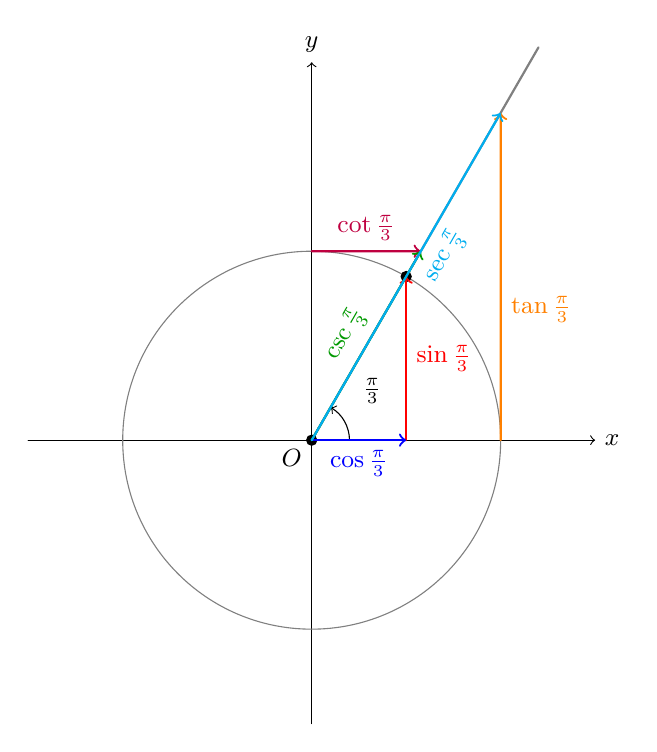
\begin{tikzpicture}[
  scale=2.4,
  line cap=round,
  font=\small
]
  % 坐标轴
  \draw[->] (-1.5,0) -- (1.5,0) node[right] {$x$};
  \draw[->] (0,-1.5) -- (0,2) node[above] {$y$};

  % 单位圆
  \draw[gray, thin] (0,0) circle(1);

  % 设定角度
  \def\theta{60}
  \pgfmathsetmacro\cs{cos(\theta)}
  \pgfmathsetmacro\sn{sin(\theta)}
  \pgfmathsetmacro\tg{tan(\theta)}
  \pgfmathsetmacro\ctg{1/tan(\theta)}

  % 关键点
  \coordinate (O) at (0,0);
  \coordinate (P) at (\cs,\sn);
  \coordinate (M) at (\cs,0);
  \coordinate (T) at (1,\tg);
  \coordinate (S) at (\ctg,1);

  % 终边
  \draw[gray, thick] (O) -- (1.2,{1.2*tan(\theta)});

  % 角度弧
  \draw[->] (0.2,0) arc (0:\theta:0.2);
  \node at (0.32,0.26) {$\frac{\pi}{3}$};

  % 原点与圆上点
  \fill (O) circle(0.03) node[below left] {$O$};
  \fill (P) circle(0.03);

  % ---- 六个三角函数 ----

  % 1. 正弦 sin(π/3) = MP (红)
  \draw[dashed, gray] (P) -- (M);
  \draw[red, thick, ->] (M) -- (P)
    node[pos=0.5, right] {$\sin\frac{\pi}{3}$};

  % 2. 余弦 cos(π/3) = OM (蓝)
  \draw[blue, thick, ->] (O) -- (M)
    node[midway, below] {$\cos\frac{\pi}{3}$};

  % 3. 正切 tan(π/3) = AT (橙)
  \draw[dashed, gray] (1,0) -- (T);
  \draw[orange, thick, ->] (1,0) -- (T)
    node[pos=0.4, right] {$\tan\frac{\pi}{3}$};

  % 4. 余切 cot(π/3) = BS (紫)
  \draw[dashed, gray] (0,1) -- (S);
  \draw[purple, thick, ->] (0,1) -- (S)
    node[pos=0.5, above] {$\cot\frac{\pi}{3}$};

  % 5. 余割 csc(π/3) = OS (绿)
  \draw[green!60!black, thick, ->] (O) -- (S)
    node[pos=0.5, sloped, above] {$\csc\frac{\pi}{3}$};

  % 6. 正割 sec(π/3) = OT (青)
  \draw[cyan, thick, ->] (O) -- (T)
    node[pos=0.6, sloped, below] {$\sec\frac{\pi}{3}$};

\end{tikzpicture}
\end{center}

我们知道，\(\sin\)，\(\cos\)，\(\tan\)在直角三角形里有它们的定义。相应的，\(\cot\)，\(\sec\)，\(\csc\)也有它们的定义。一般地，在直角三角形中，我们定义\(\cot=\frac{\text{邻边}}{\text{对边}}\)，\(\sec=\frac{\text{斜边}}{\text{邻边}}\)，\(\csc=\frac{\text{斜边}}{\text{对边}}\)。细心的你也许已经发现了，其实\(\cot\)就是\(\tan\)的倒数，\(\sec\)就是\(\cos\)的倒数，\(\csc\)就是\(\sin\)的倒数。也就是说，我们只需要用高中计算\(\sin\)，\(\cos\)，\(\tan\)的方法，再记住它们的倒数关系，就能很快的算出\(\cot\)，\(\sec\)，\(\csc\)了。同样的，我们从直角三角形推广到全体实数，就引入了单位圆定义。高中的单位圆定义了\(\sin\)，\(\cos\)，\(\tan\)，这次我们把\(\cot\)，\(\sec\)，\(\csc\)的定义一起加上了。

不过，我们主要使用的还是 $\sin$，$\cos$，$\tan$ 这三个，$\sec$，$\cot$，$\csc$ 不能说不用，只是出现得比较少。

\begin{myexample}
  利用单位圆定义，求 $\sec\frac{\pi}{3}$、$\cot\frac{\pi}{3}$、$\csc\frac{\pi}{3}$ 的值。

角 $\frac{\pi}{3}$ 的终边与单位圆的交点为 $P\!(\frac{1}{2}, \frac{\sqrt{3}}{2})$。因此：

\[
\sin\frac{\pi}{3} = \frac{\sqrt{3}}{2},\quad 
\cos\frac{\pi}{3} = \frac{1}{2},\quad 
\tan\frac{\pi}{3} = \frac{\sin\frac{\pi}{3}}{\cos\frac{\pi}{3}} = \sqrt{3}
\]

利用倒数关系可得：
\[
\sec\frac{\pi}{3} = \frac{1}{\cos\frac{\pi}{3}} = 2,\quad 
\csc\frac{\pi}{3} = \frac{1}{\sin\frac{\pi}{3}} = \frac{2\sqrt{3}}{3},\quad 
\cot\frac{\pi}{3} = \frac{1}{\tan\frac{\pi}{3}} = \frac{\sqrt{3}}{3}
\]

\end{myexample}

这正是图上各个三角函数的值。在单位圆定义里，它们表示的是线段的长度。

常见的特殊角的三角函数值需要牢记。这些值不需要死记硬背。画一个单位圆，标出各特殊角对应的点坐标，$\sin$ 读纵坐标、$\cos$ 读横坐标、$\tan$ 读纵横之比，剩下的就能全部推出来。


\subsection{三角函数公式}

三角函数有很多公式，例如刚刚说到的倒数关系：
\begin{theorem}{三角函数的倒数关系}{}
\[
\sin\theta \cdot \csc\theta = 1,\quad
\cos\theta \cdot \sec\theta = 1,\quad
\tan\theta \cdot \cot\theta = 1
\]
\end{theorem}

还有平方关系：
\begin{theorem}{三角函数的平方关系}{}
\[
\sin^2\theta + \cos^2\theta = 1,\quad
1 + \tan^2\theta = \sec^2\theta,\quad
1 + \cot^2\theta = \csc^2\theta
\]
\end{theorem}

第一个公式是勾股定理的三角版本，后面两个是第一个两边分别除以 $\cos^2\theta$ 和 $\sin^2\theta$ 得到的。

接着是诱导公式。诱导公式用来把任意角化简为 $0$ 到 $\frac{\pi}{2}$ 之间的角。核心规律是“奇变偶不变，符号看象限”。具体的操作我们假定读者高中已经掌握，所以我们不再赘述。

\begin{theorem}{三角函数的诱导公式}{}
\[
\begin{aligned}
\sin(-\theta) &= -\sin\theta, & \sin(\frac{\pi}{2} \pm \theta) &= \cos\theta, & \sin(\pi \pm \theta) &= \mp\sin\theta \\[6pt]
\cos(-\theta) &= \cos\theta, & \cos(\frac{\pi}{2} \pm \theta) &= \mp\sin\theta, & \cos(\pi \pm \theta) &= -\cos\theta \\[6pt]
\tan(-\theta) &= -\tan\theta, & \tan(\frac{\pi}{2} \pm \theta) &= \mp\cot\theta, & \tan(\pi \pm \theta) &= \pm\tan\theta \\[6pt]
\cot(-\theta) &= -\cot\theta, & \cot(\frac{\pi}{2} \pm \theta) &= \mp\tan\theta, & \cot(\pi \pm \theta) &= \pm\cot\theta \\[6pt]
\sec(-\theta) &= \sec\theta, & \sec(\frac{\pi}{2} \pm \theta) &= \mp\csc\theta, & \sec(\pi \pm \theta) &= -\sec\theta \\[6pt]
\csc(-\theta) &= -\csc\theta, & \csc(\frac{\pi}{2} \pm \theta) &= \sec\theta, & \csc(\pi \pm \theta) &= \mp\csc\theta
\end{aligned}
\]
\end{theorem}



然后是和差公式：
\begin{theorem}{三角函数的和差公式}{}
\[
\begin{aligned}
\sin(\alpha \pm \beta) &= \sin\alpha\cos\beta \pm \cos\alpha\sin\beta \\
\cos(\alpha \pm \beta) &= \cos\alpha\cos\beta \mp \sin\alpha\sin\beta \\
\tan(\alpha \pm \beta) &= \frac{\tan\alpha \pm \tan\beta}{1 \mp \tan\alpha\tan\beta} \\
\cot(\alpha \pm \beta) &= \frac{\cot\alpha\cot\beta \mp 1}{\cot\beta \pm \cot\alpha} \\
\sec(\alpha \pm \beta) &= \frac{\sec\alpha\sec\beta}{1 \mp \tan\alpha\tan\beta} \\
\csc(\alpha \pm \beta) &= \frac{\csc\alpha\csc\beta}{\cot\beta \pm \cot\alpha}
\end{aligned}
\]
\end{theorem}

然后是倍角公式：
\begin{theorem}{三角函数的倍角公式}{}
\[
\begin{aligned}
\sin 2\theta &= 2\sin\theta\cos\theta\\
\cos 2\theta &= \cos^2\theta - \sin^2\theta = 2\cos^2\theta - 1 = 1 - 2\sin^2\theta\\
\tan 2\theta &= \frac{2\tan\theta}{1 - \tan^2\theta}\\
\cot 2\theta &= \frac{\cot^2\theta - 1}{2\cot\theta}\\
\sec 2\theta &= \frac{\sec^2\theta}{1 - \tan^2\theta}\\
\csc 2\theta &= \frac{\csc^2\theta}{2\cot\theta}
\end{aligned}
\]
\end{theorem}

它们可以由和角公式直接得到。

然后是半角公式：
\begin{theorem}{三角函数的半角公式}{}
\[
\begin{aligned}
\sin\frac{\theta}{2} &= \pm \sqrt{\frac{1 - \cos\theta}{2}}\\
\cos\frac{\theta}{2} &= \pm \sqrt{\frac{1 + \cos\theta}{2}}\\
\tan\frac{\theta}{2} &= \pm \sqrt{\frac{1 - \cos\theta}{1 + \cos\theta}} = \frac{\sin\theta}{1 + \cos\theta} = \frac{1 - \cos\theta}{\sin\theta}\\
\cot\frac{\theta}{2} &= \pm \sqrt{\frac{1 + \cos\theta}{1 - \cos\theta}} = \frac{\sin\theta}{1 - \cos\theta} = \frac{1 + \cos\theta}{\sin\theta}\\
\sec\frac{\theta}{2} &= \pm \sqrt{\frac{2\sec\theta}{\sec\theta + 1}} = \pm \sqrt{\frac{2}{1 + \cos\theta}}\\
\csc\frac{\theta}{2} &= \pm \sqrt{\frac{2\csc\theta}{\csc\theta - \cot\theta}} = \pm \sqrt{\frac{2}{1 - \cos\theta}}
\end{aligned}
\]
\end{theorem}
它们是倍角公式的逆用。其中正负由\(\frac{\theta }{2}\)所在的象限决定。

然后是降幂公式：
\begin{theorem}{三角函数的降幂公式}{}
\[
\begin{aligned}
\sin^2\theta &= \frac{1 - \cos 2\theta}{2}, & \cos^2\theta &= \frac{1 + \cos 2\theta}{2} \\[6pt]
\tan^2\theta &= \frac{1 - \cos 2\theta}{1 + \cos 2\theta}, & \cot^2\theta &= \frac{1 + \cos 2\theta}{1 - \cos 2\theta} \\[6pt]
\sec^2\theta &= \frac{2}{1 + \cos 2\theta}, & \csc^2\theta &= \frac{2}{1 - \cos 2\theta}
\end{aligned}
\]
\end{theorem}

半角公式移项就是降幂公式，常用于积分中把高次三角幂降为低次。

其实这些公式不用特别记忆，需要的时候回来看一下，多用一下就记住了。如果有些公式记不住，那就说明不常用，不记也罢。

\subsection{反三角函数}

反三角函数，顾名思义，就是三角函数反过来。三角函数是已知角，求对应比值，反三角函数就是已知比值，求对应角度。例如 $\sin\theta = \frac{1}{2}$，求 $\theta$ 等于多少？你马上能说出来 $\theta=\frac{\pi}{6}$。但注意，$\sin\frac{5\pi}{6}$ 也等于 $\frac{1}{2}$，$\sin\frac{13\pi}{6}$ 也等于 $\frac{1}{2}$。这就产生了一点问题，我们知道，在函数的概念里，一个$x$对应一个$y$。现在的$x$是$\frac{1}{2}$，但是对应了$\frac{\pi}{6}$，$\frac{5\pi}{6}$，$\frac{13\pi}{6}$，甚至更多的$y$。因此，反三角函数必须把值域限制在一个特定区间内，使得一个$x$必须对应一个$y$，否则一个比值会对应无穷多个角，就不是“函数”了。

最常用的三个反三角函数是反正弦、反余弦、反正切。

\begin{definition}{反正弦函数}{}
设 $x \in [-1, 1]$，若存在唯一的 $y \in [-\frac{\pi}{2}, \frac{\pi}{2}]$ 使得 $\sin y = x$，
则称 $y$ 为 $x$ 的反正弦，记作
\[
y = \arcsin x
\]
其中，函数 $y = \arcsin x$ 的定义域为 $[-1, 1]$，值域为 $[-\frac{\pi}{2}, \frac{\pi}{2}]$。
\end{definition}

例如 $\arcsin\frac{1}{2} = \frac{\pi}{6}$，$\arcsin(-1) = -\frac{\pi}{2}$，$\arcsin 0 = 0$。我们这里值域取的是 $\sin$ 在 $[-\frac{\pi}{2}, \frac{\pi}{2}]$ 上的那一段，这恰好是 $\sin$ 单调递增的区间，保证了一一对应。

同理，我们有：

\begin{definition}{反余弦函数}{}
设 $x \in [-1, 1]$，若存在唯一的 $y \in [0, \pi]$ 使得 $\cos y = x$，
则称 $y$ 为 $x$ 的反余弦，记作
\[
y = \arccos x
\]
其中，函数 $y = \arccos x$ 的定义域为 $[-1, 1]$，值域为 $[0, \pi]$。
\end{definition}

例如 $\arccos\frac{1}{2} = \frac{\pi}{3}$，$\arccos(-1) = \pi$，$\arccos 0 = \frac{\pi}{2}$。$\cos$ 在 $[0, \pi]$ 上单调递减。

同理，我们有：

\begin{definition}{反正切函数}{}
设 $x \in \mathbb{R}$，若存在唯一的 $y \in (-\frac{\pi}{2}, \frac{\pi}{2})$ 使得 $\tan y = x$，
则称 $y$ 为 $x$ 的反正切，记作
\[
y = \arctan x
\]
其中，函数 $y = \arctan x$ 的定义域为 $\mathbb{R}$，值域为 $(-\frac{\pi}{2}, \frac{\pi}{2})$。
\end{definition}

例如 $\arctan 1 = \frac{\pi}{4}$，$\arctan\sqrt{3} = \frac{\pi}{3}$，$\arctan 0 = 0$。剩下三个反三角函数也是类似的定义，不过它们实在是出现得太少，我们省略了，需要时查表即可。

同样的，反三角函数也有它们的公式。不过实际情况几乎用不到，而且也不在我们微积分的讨论范围内，所以我们此处也省略不讲了。

